\section{Material Aligned}\label{sec:mat_aligned}

\subsection{Neutron transport with larger geometry}
This section documents the neutron flux obtained using the geometry shown 
in Figure \ref{fig:large_geom}.
The geometry on top is the original geometry with two volumes used in the 
mesh-based neutron transport run. 
The geometry at the bottom of Figure \ref{fig:large_geom} has a mesh laid 
on top. The cell-based geometry was created using the original two volumes
geometry and subdiving it to align with the mesh seem in gray in the bottom 
geometry. 

\begin{figure}[!h]
    \begin{subfigure}{1\textwidth}
        \centering
        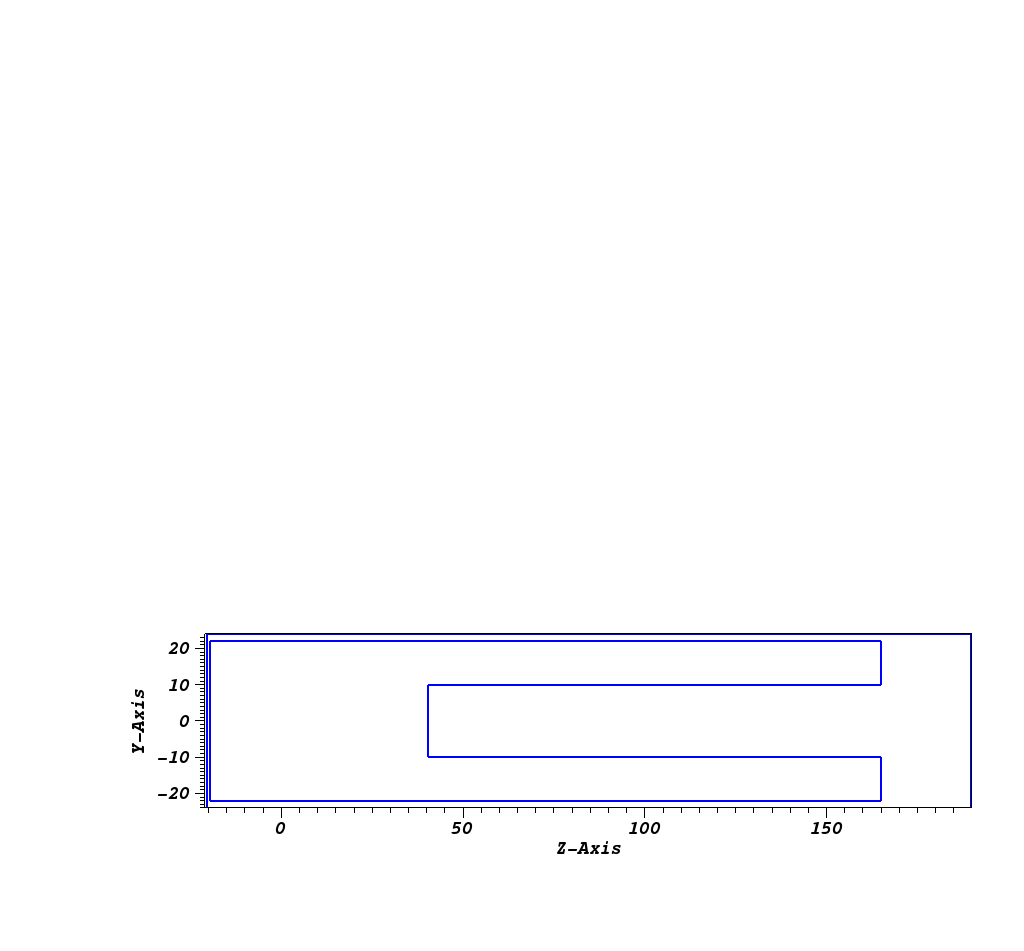
\includegraphics[scale=0.4, trim={4cm 3cm 1cm 22cm}, clip]{figs/mesh_geom_larger.png}
        \caption{}
        \label{fig:large_geom1}
    \end{subfigure}
    \begin{subfigure}{1\textwidth}
        \centering
        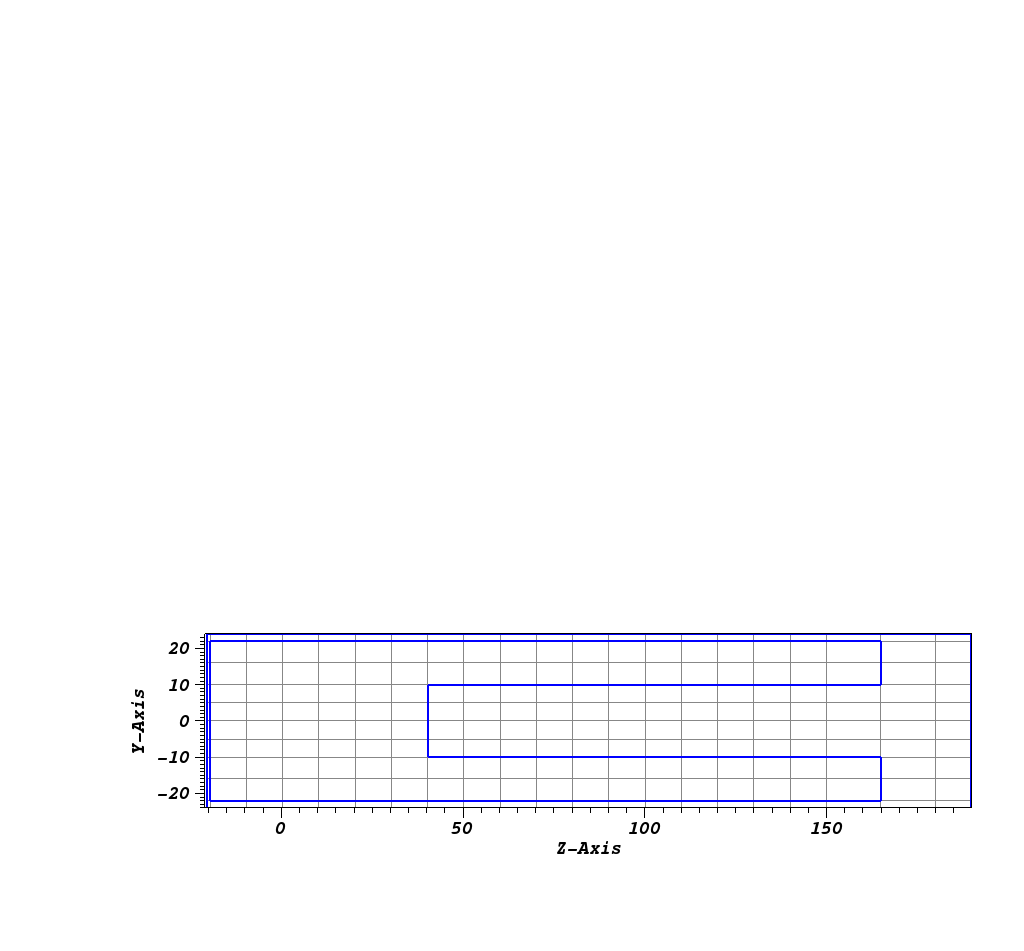
\includegraphics[scale=0.4, trim={4cm 3cm 1cm 22cm}, clip]{figs/mesh_geom_mesh_larger.png}
        \caption{}
        \label{fig:large_geom2}
    \end{subfigure}
    \caption{Large geometry with two volumes in blue and mesh in gray}
    \label{fig:large_geom}
\end{figure}

The source used was positioned on the left side of the geometry and it 
is the complicated source originally used for \gls{sns}. 


After the first tranport with 2E8 particles, the neutron flux was examined. 
The neutron flux ratio between the mesh-based and cell-based workflows 
is shown in Figure \ref{fig:n_ratio_larger}. 
This figure shows that the netron fluxes obtained with each workflow 
compare well at the front of the geometry with a high degree of certainty. 
As we move toward the back of the geometry, the certainty on the 
ratio lessens. 
Because the the fluxes are not able to be matched up with high certainty, 
the rest of the workflow was not completed. 
Instead a smaller geometry was used with a simpler source.  

\begin{figure}
    \begin{subfigure}{0.1\textwidth}
        \centering
        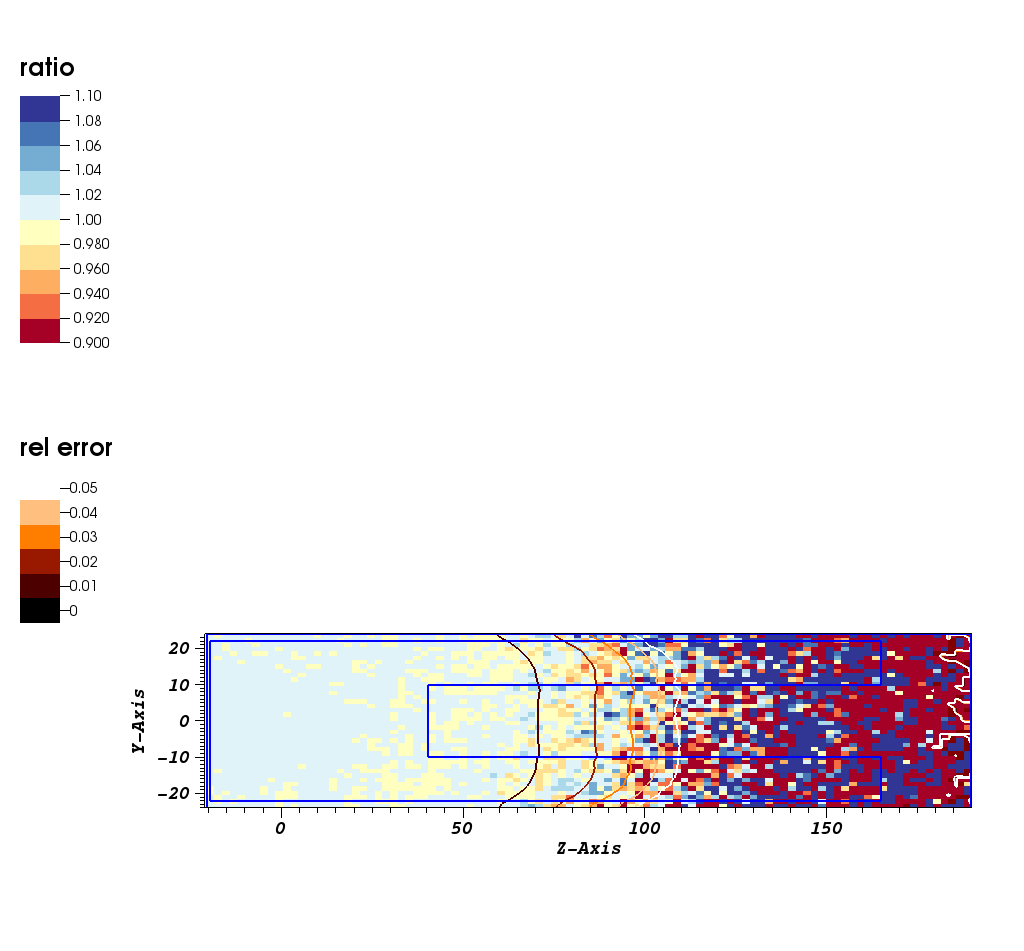
\includegraphics[scale=0.35, trim={0cm 20cm 31cm 2cm}, clip]{figs/ratio_nflux_larger.png}
    \end{subfigure}
    \begin{subfigure}{0.1\textwidth}
        \centering
        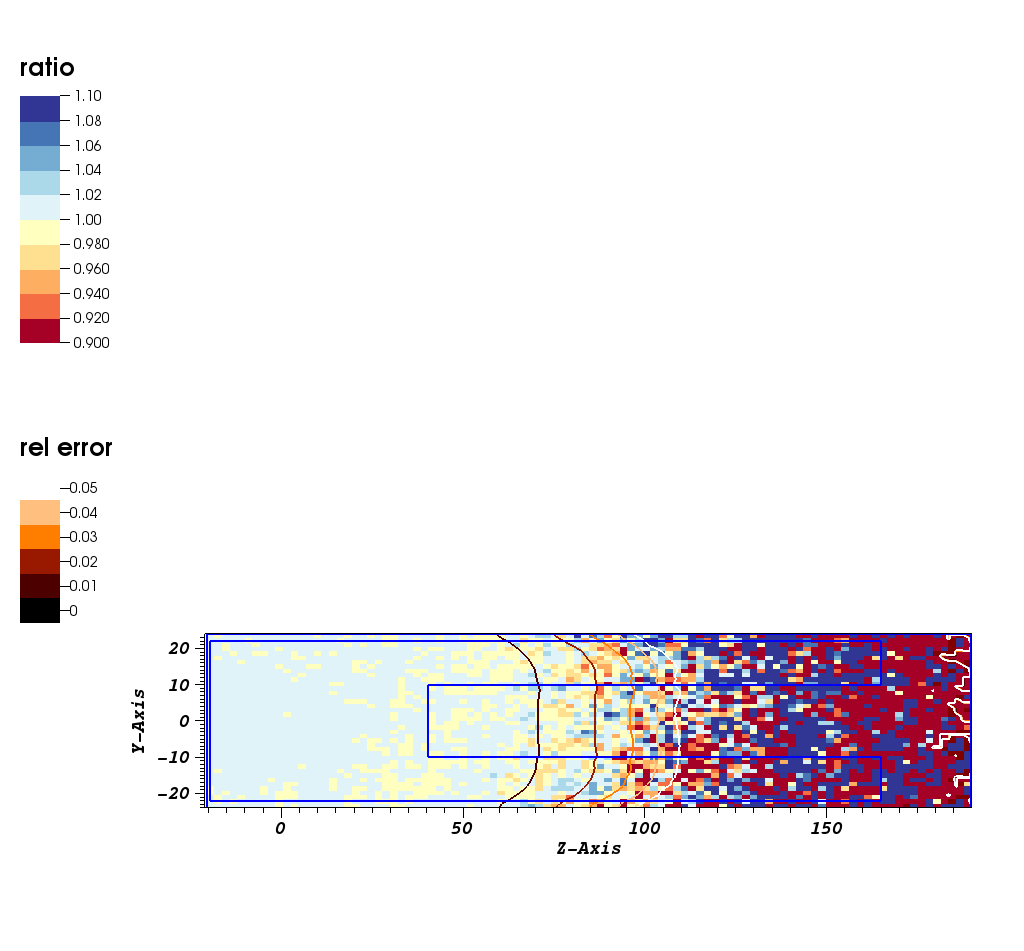
\includegraphics[scale=0.35, trim={0cm 6.1cm 32cm 15cm}, clip]{figs/ratio_nflux_larger.png}
    \end{subfigure}
    \begin{subfigure}{0.79\textwidth}
        \centering
        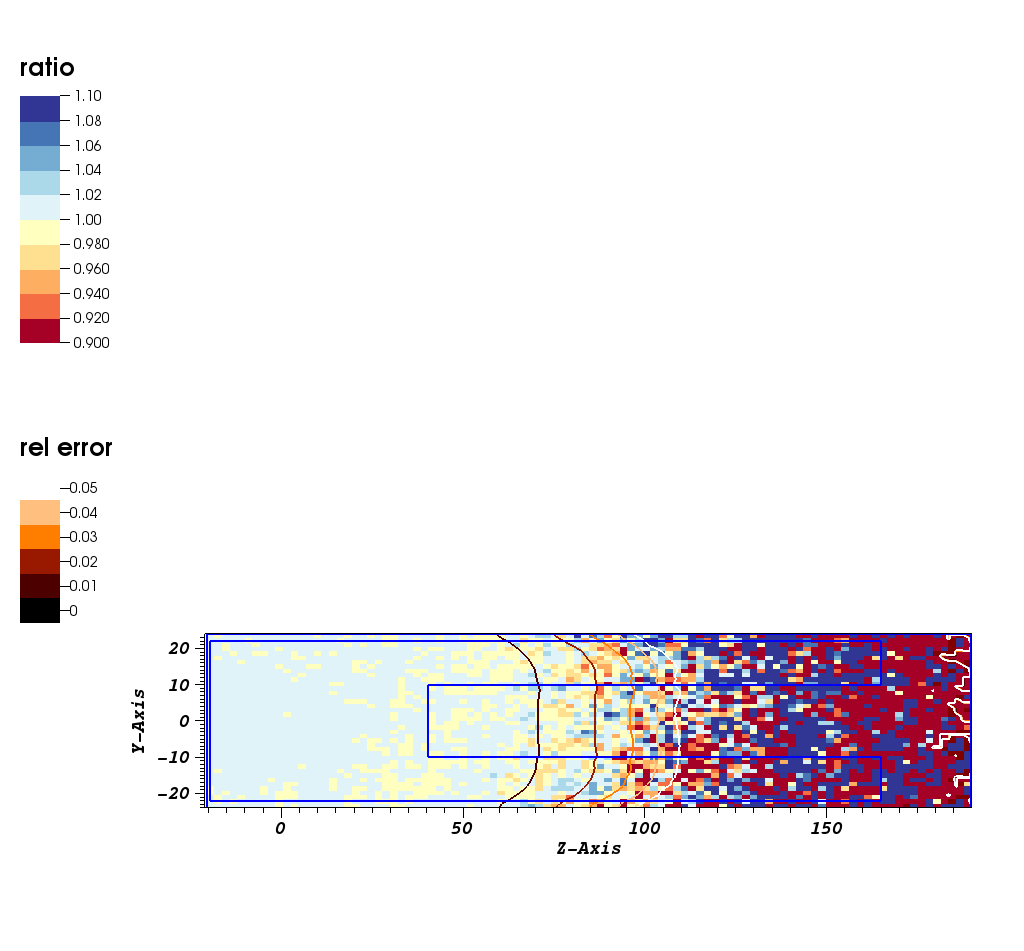
\includegraphics[scale=0.5, trim={4cm 2cm 1cm 22cm}, clip]{figs/ratio_nflux_larger.png}
    \end{subfigure}
    \caption{Neutron flux ratio [Mesh/Cell]}
    \label{fig:n_ratio_larger}
\end{figure}

\subsection{Smaller Geometry}
The smaller geometry is a geometry that was been reduced by 1/32 in volume. 
The dimensions of the outer steel are 7 cm x 12 cm x 52.75 cm. 
The geometry can be seen in Figure \ref{fig:smaller_geom1}. 
Figure \ref{fig:smaller_geom2} shows the material aligned mesh used in 
the mesh-based workflow. 
For the cell-based workflow, the geometry in Figure \ref{fig:smaller_geom1}
was subdivided to match the mesh in Figure \ref{fig:smaller_geom2}. 
\begin{figure}[!h]
    \begin{subfigure}{1\textwidth}
        \centering
        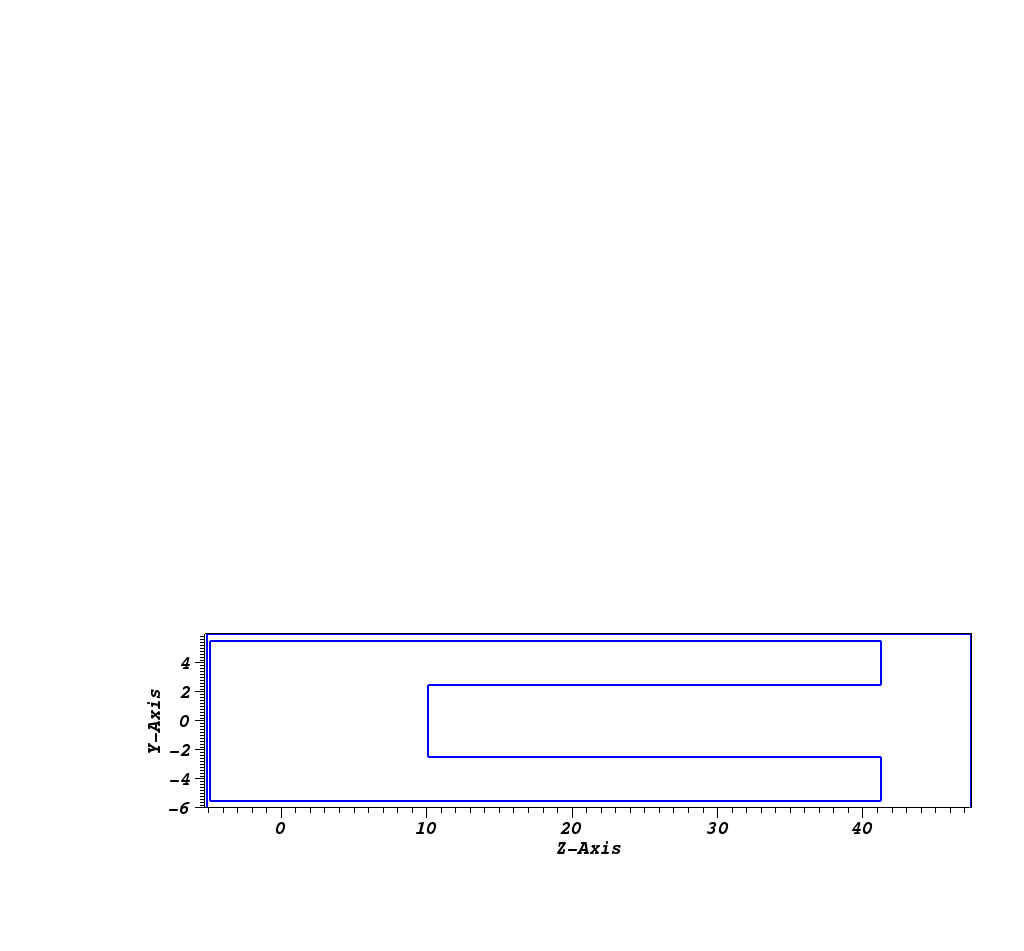
\includegraphics[scale=0.4, trim={4cm 3cm 1cm 22cm}, clip]{figs/mesh_geom.png}
        \caption{}
        \label{fig:smaller_geom1}
    \end{subfigure}
    \begin{subfigure}{1\textwidth}
        \centering
        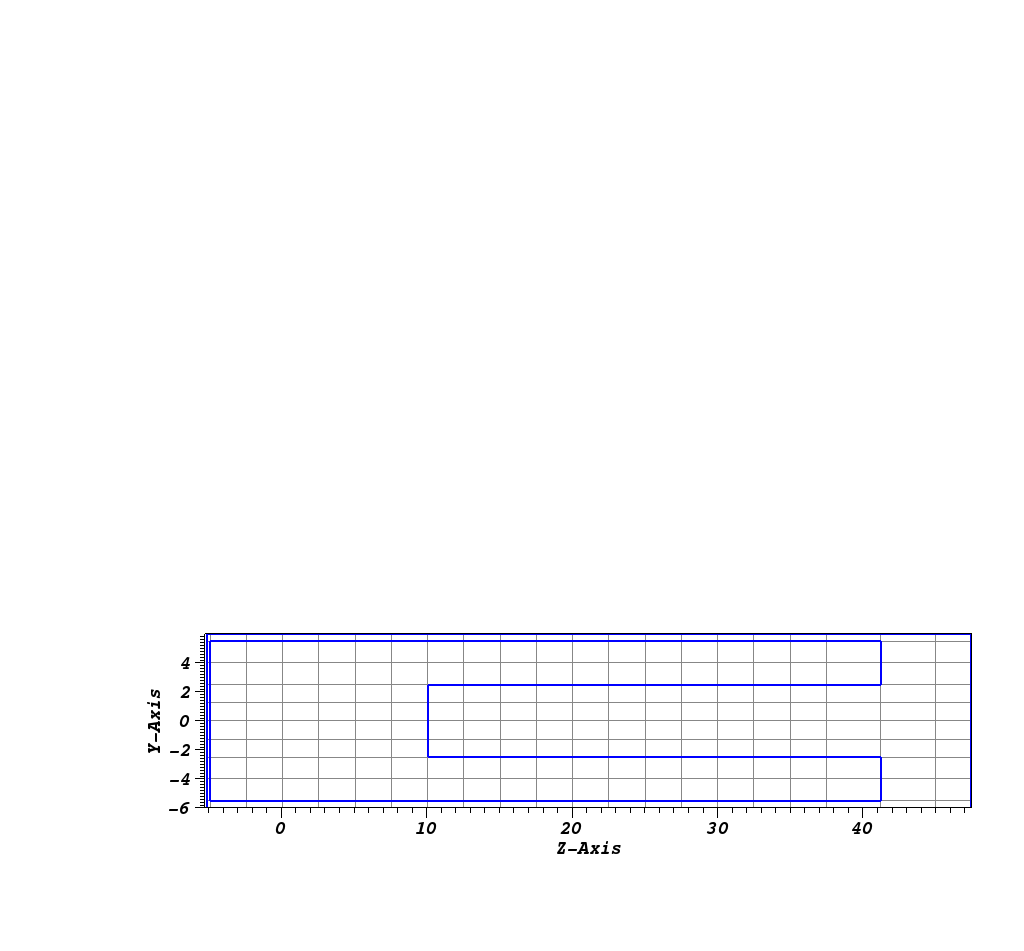
\includegraphics[scale=0.4, trim={4cm 3cm 1cm 22cm}, clip]{figs/mesh_geom_mesh.png}
        \caption{}
        \label{fig:smaller_geom2}
    \end{subfigure}
    \caption{Smaller geometry with two volumes in blue and mesh in gray}
    \label{fig:smaller_geom}
\end{figure}
%
The source used was a disk source perpendicular to the z-axis at ???
CHECK THE POSITION 
uniformly emitting 1 GeV protons monodirectionally in z-direction.
\begin{figure}
    \begin{subfigure}{0.1\textwidth}
        \centering
        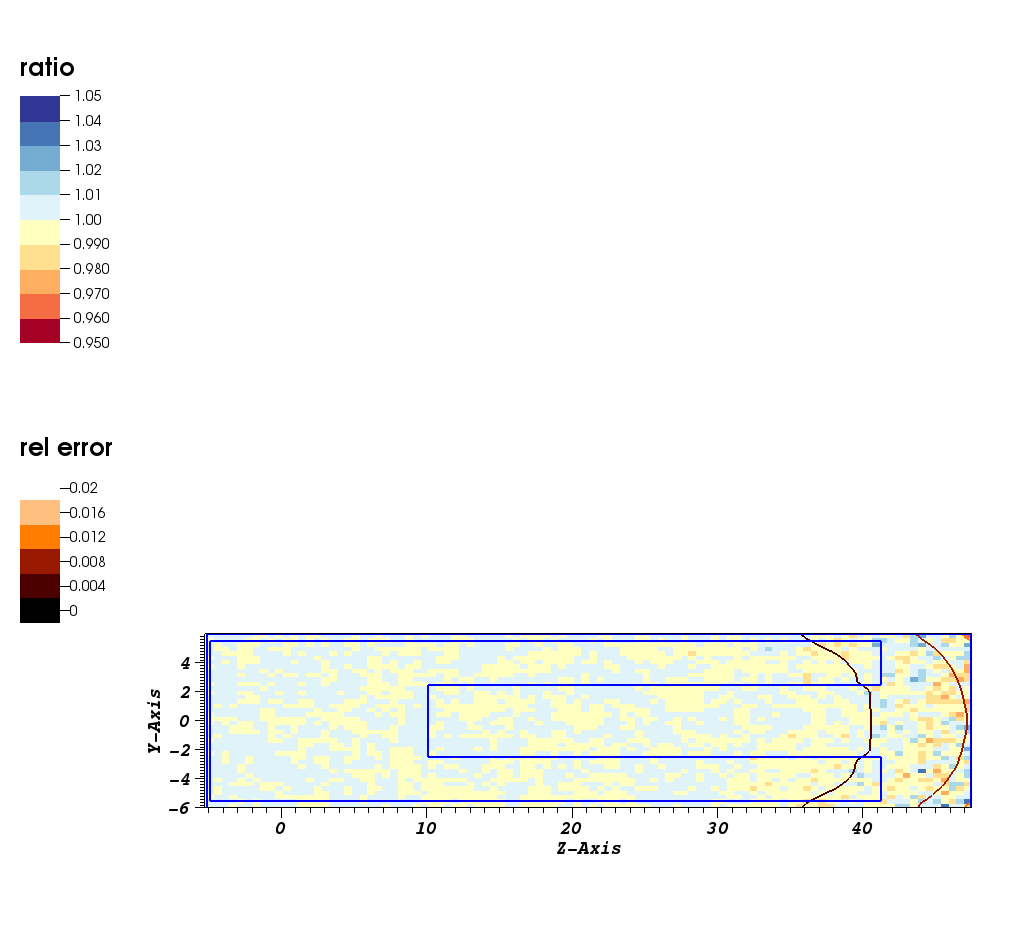
\includegraphics[scale=0.35, trim={0cm 20cm 31cm 2cm}, clip]{figs/ratio_nflux.png}
    \end{subfigure}
    \begin{subfigure}{0.1\textwidth}
        \centering
        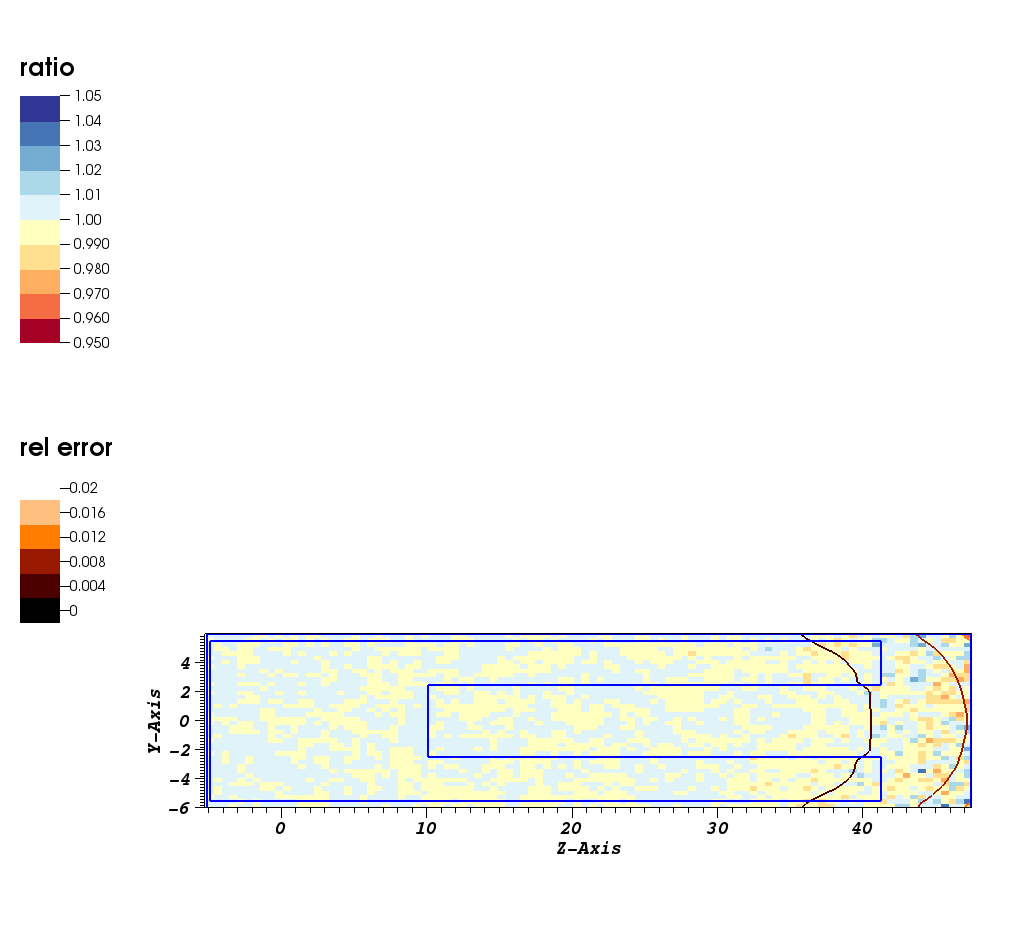
\includegraphics[scale=0.35, trim={0cm 6.1cm 32cm 15cm}, clip]{figs/ratio_nflux.png}
    \end{subfigure}
    \begin{subfigure}{0.79\textwidth}
        \centering
        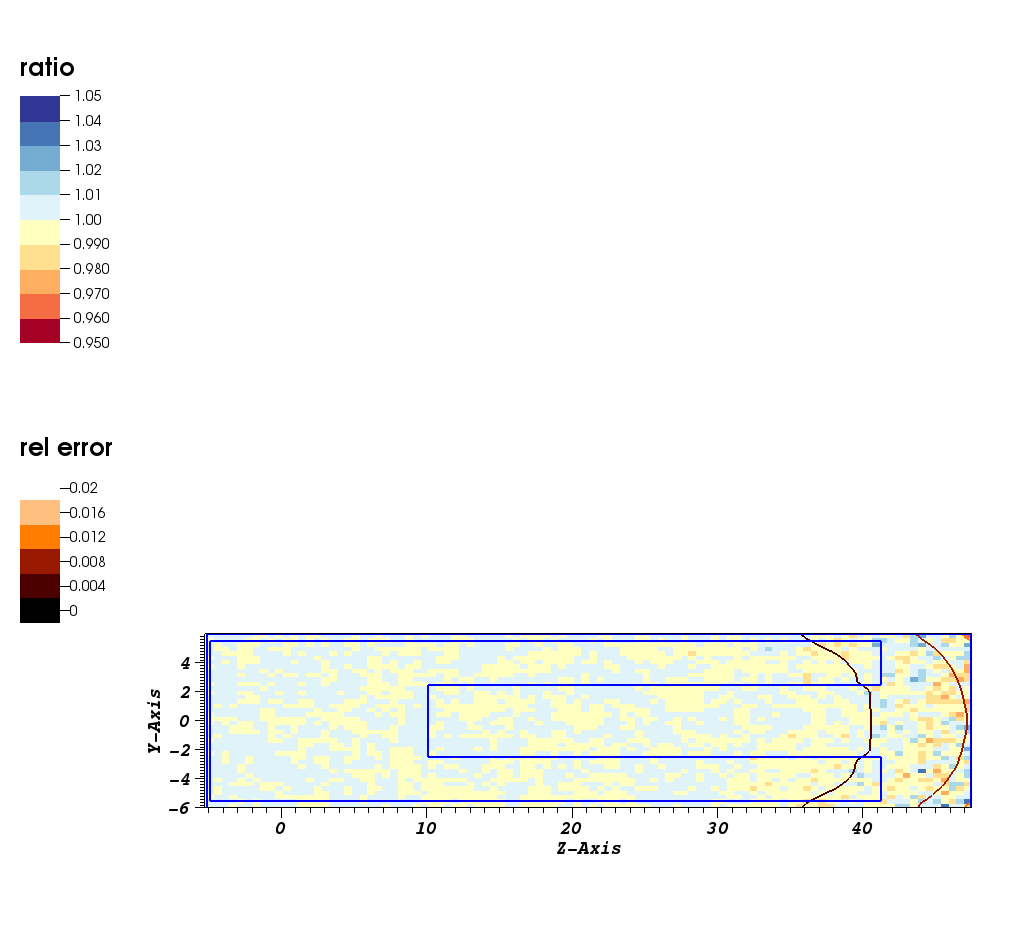
\includegraphics[scale=0.5, trim={4cm 2cm 1cm 22cm}, clip]{figs/ratio_nflux.png}
    \end{subfigure}
    \caption{Neutron flux ratio [Mesh/Cell]}
    \label{fig:n_ratio_smaller}
\end{figure}
 

The neutron flux was inspected and the ratio between the mesh-based and 
cell-based workflow is shown in Figure \ref{fig:n_ratio_smaller}. 
This figure shows that the neutron flux for both workflows are similar 
discrepancies less than 5\% and statistical errors less than 2 \%. 

The photon transport was run with 1E10 particles. 
For the cell workflow the photon source SDEF card was divided into 5 parts 
because of the number of volumetric cells involved. 
\begin{figure}
    \begin{subfigure}{0.1\textwidth}
        \centering
        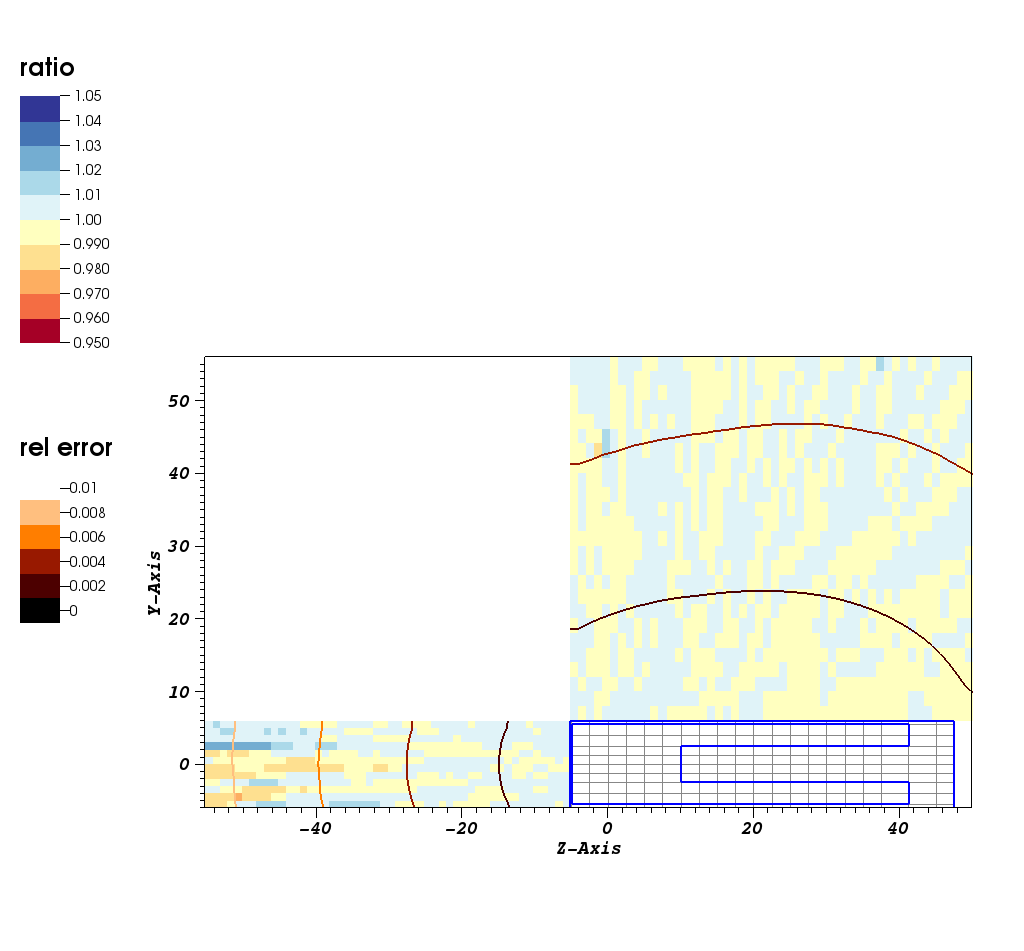
\includegraphics[scale=0.35, trim={0cm 20cm 31cm 2cm}, clip]{figs/dose_ratio_mat_aligned.png}
    \end{subfigure}
    \begin{subfigure}{0.1\textwidth}
        \centering
        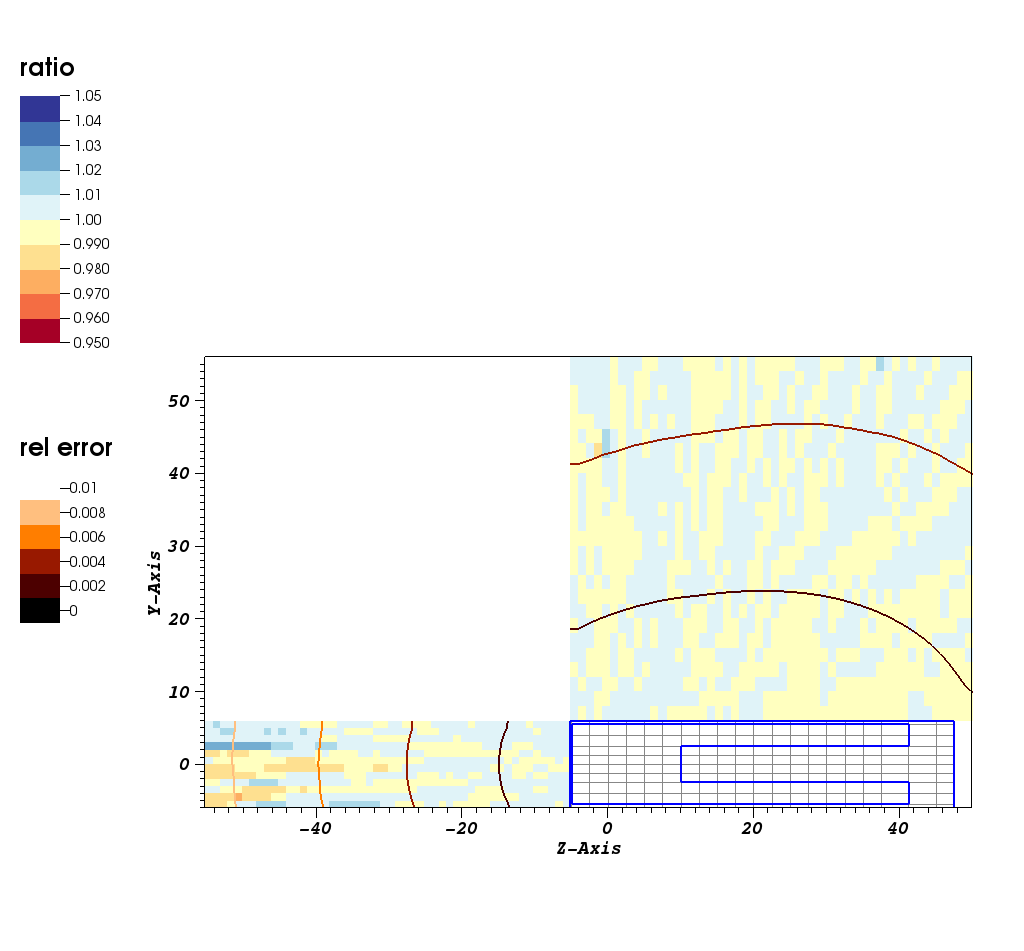
\includegraphics[scale=0.35, trim={0cm 6.1cm 32cm 15cm}, clip]{figs/dose_ratio_mat_aligned.png}
    \end{subfigure}
    \begin{subfigure}{0.79\textwidth}
        \centering
        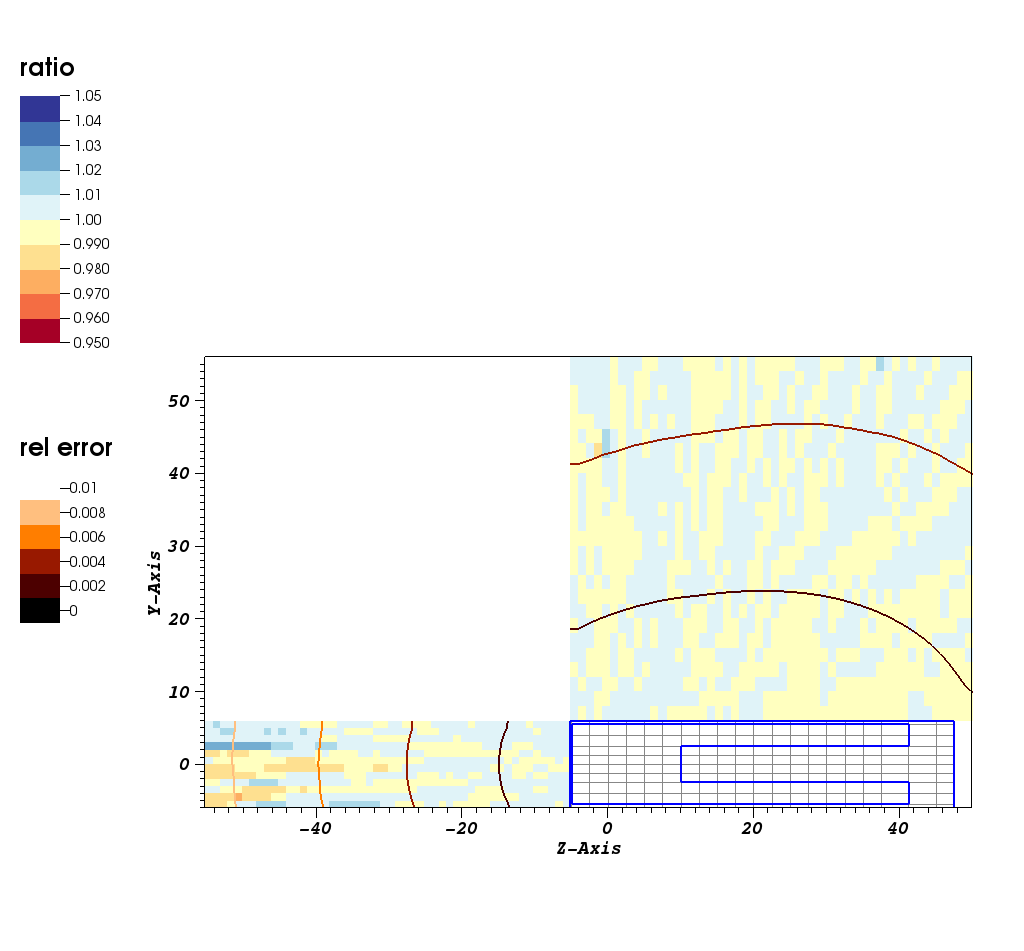
\includegraphics[scale=0.5, trim={4cm 2cm 1cm 12cm}, clip]{figs/dose_ratio_mat_aligned.png}
    \end{subfigure}
    \caption{Dose rate ratio [Mesh/Cell]}
    \label{fig:n_ratio_larger}
\end{figure}




\begin{figure}[!h]
    \centering
    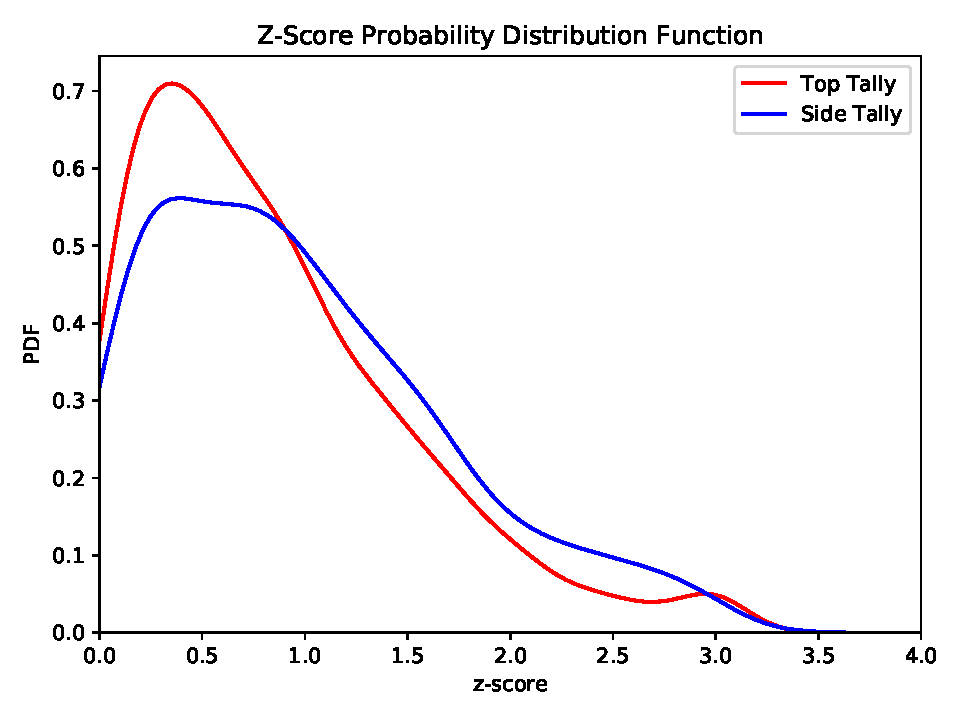
\includegraphics[scale=0.6, trim={0cm 0cm 0cm 0cm}, clip]{figs/dose_pdf.pdf}
    \caption{PDF}
    \label{fig:dose_pdf}
\end{figure}
\begin{figure}[!h]
    \centering
    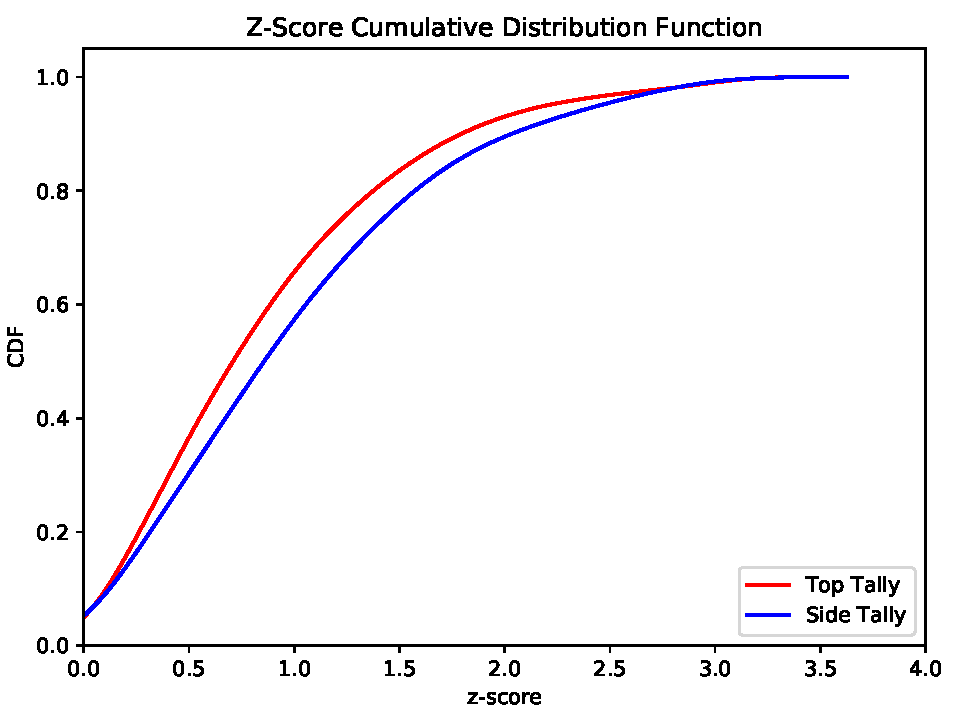
\includegraphics[scale=0.6, trim={0cm 0cm 0cm 0cm}, clip]{figs/dose_cdf.pdf}
    \caption{CDF}
    \label{fig:dose_cdf}
\end{figure}

\begin{table}[]
    \centering
    \begin{tabular}{|r|r|r|}
    \hline
               & Top Tally & Side Tally \\ \hline
    z $\leq$ 1 & 66.5\%    & 58.3\%     \\ \hline
    z $\leq$ 2 & 93.1\%    & 89.8\%     \\ \hline
    z $\leq$ 3 & 98.3\%    & 99.7\%     \\ \hline
    \end{tabular}
\end{table}